
\section{Углы} 

\subsection*{Предварительные понятия}

\paragraph{Угол.}\label{1938/13}
Фигура, образованная двумя лучами, исходящими из одной точки, называется \rindex{угол}\textbf{углом}.
Полупрямые, образующие угол, называются \rindex{сторона!угла}\textbf{сторонами}, а точка, из которой они исходят, — \rindex{вершина!угла}\textbf{вершиной угла}.
Стороны следует представлять себе неограниченно продолженными от вершины.

\begin{wrapfigure}{o}{31 mm}
\centering
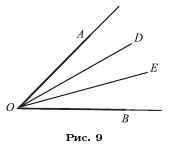
\includegraphics{mppics/ris-9}
\caption{}\label{1938/ris-9}
\end{wrapfigure}

Угол обыкновенно обозначается тремя большими буквами, из которых средняя ставится у вершины, а крайние — у каких-нибудь точек сторон;
например, говорят:
«угол $AOB$» или «угол $BOA$» (рис.~\ref{1938/ris-9}).
Но можно обозначить угол и одной буквой, поставленной у вершины, если при этой вершине нет других углов.
Мы иногда будем обозначать угол цифрой, поставленной внутри угла около вершины.

Стороны угла разделяют всю плоскость, в которой лежит этот угол, на две области.
Одна из них называется \rindex{внутренняя область угла}\textbf{внутренней областью угла}, другая — \rindex{внешняя область угла}\textbf{внешней его областью}.
Обычно внутренней областью считается та, в которой целиком помещается отрезок, соединяющей две любые точки, взятые на сторонах угла, например точки $A$ и $B$ на сторонах угла $AOB$ (рис.~\ref{1938/ris-9}).
Но иногда приходится считать внутренней областью угла другую часть плоскости.
В этих случаях обычно делается специальное указание, какая область плоскости считается внутренней областью угла.

На рис.~\ref{1938/ris-10} представлены раздельно оба случая.
Внутренней областью угла в каждом случае служит заштрихованная часть плоскости.
Если из вершины угла (рис.~\ref{1938/ris-9}) проведём внутри него какие-нибудь прямые $OD, OE,\dots$, то образовавшиеся при этом углы $AOD$, $DOE$, $EOB,\dots$, рассматриваются как части угла $AOB$.

\begin{figure}[!ht]
\centering
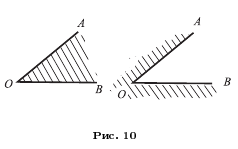
\includegraphics{mppics/ris-10}
\caption{}\label{1938/ris-10}
\end{figure}

Слово «угол» при записи заменяется часто знаком $\angle$.
Например, вместо «угол $AOB$» обычно пишут:
$\angle AOB$.

\paragraph{Равенство и неравенство углов.}\label{1938/14}
В соответствии с общим определением равенства геометрических фигур (§~\ref{1938/1}) \emph{два угла считаются равными, если при наложении они могут совместиться.}

\begin{figure}[h]
\centering
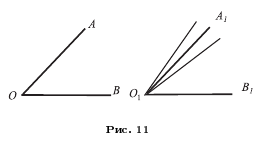
\includegraphics{mppics/ris-11}
\caption{}\label{1938/ris-11}
\end{figure}

{\sloppy
Положим, например, что мы накладываем угол $AOB$ на угол $A_1O_1B_1$ (рис.~\ref{1938/ris-11}) так, чтобы вершина $O$ совпала с $O_1$, сторона $OB$ пошла по $O_1B_1$ и чтобы внутренние области обоих углов были расположены по одну сторону от прямой $O_1B_1$.
Если при этом сторона $OA$ совместится с $O_1A_1$, то углы равны;
если же $OA$ пойдёт внутри угла $A_1O_1B_1$ или же вне его, то углы не равны, причём тот из них будет меньше, который составит часть другого угла.

}

\begin{figure}[!ht]
\centering
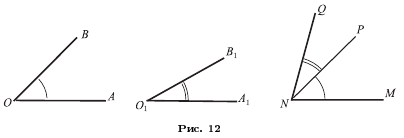
\includegraphics{mppics/ris-12}
\caption{}\label{1938/ris-12}
\end{figure}

\paragraph{Сумма углов.}\label{1938/15}
\rindex{сумма углов}
Суммой углов $AOB$ и $A_1O_1B_1$ (рис.~\ref{1938/ris-12}) называется такой угол, который получится следующим образом.
Строим угол $MNP$, равный первому данному углу $AOB$, и к нему пристраиваем угол $PNQ$, равный другому данному углу $A_1O_1B_1$ так, чтобы у обоих углов оказалась общая вершина $N$ и общая сторона $NP$ и чтобы внутренние области углов были расположены по разные стороны от общей стороны $NP$.
Тогда угол $MNQ$, называется суммой углов $AOB$ и $A_1O_1B_1$.
Внутренней областью этого угла служит та область плоскости, которая образована совокупностью внутренних областей складываемых углов.
Это та область, в которой лежит общая сторона ($NP$) складываемых углов.
Подобным образом может быть составлена сумма трёх и более углов.

\begin{wrapfigure}{o}{35 mm}
\vskip-4mm
\centering
\includegraphics{mppics/ris-ru-13}
\caption{}\label{1938/ris-13}
\vskip-4mm
\end{wrapfigure}


Сумма углов, как и сумма отрезков, обладает свойствами переместительным и сочетательным.
Часто приходится говорить о такой полупрямой, которая делит данный угол пополам;
такой полупрямой дали особое название:
\rindex{биссектриса}\textbf{биссектриса} (рис.~\ref{1938/ris-13}).


\paragraph{Расширение понятия об угле.}\label{1938/16}
При нахождении суммы углов могут представиться некоторые особые случаи, которые полезно рассмотреть отдельно.

1.
Может случиться, что после сложения нескольких углов, например трёх:
$AOB$, $BOC$ и $COD$ (рис.~\ref{1938/ris-14}), сторона $OD$ угла $COD$ составит продолжение стороны $OA$ угла $AOB$.
Мы получим тогда фигуру, образованную двумя полупрямыми ($OA$ и $OD$), исходящими из одной точки ($O$) и составляющими продолжение одна другой.
Такую фигуру принято тоже называть углом (\rindex{развёрнутый угол}\textbf{развёрнутым}).

\begin{figure}[!ht]
\begin{minipage}{.48\textwidth}
\centering
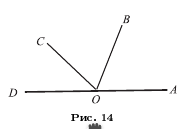
\includegraphics{mppics/ris-14}
\end{minipage}\hfill
\begin{minipage}{.48\textwidth}
\centering
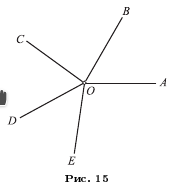
\includegraphics{mppics/ris-15}
\end{minipage}

\medskip

\begin{minipage}{.48\textwidth}
\centering
\caption{}\label{1938/ris-14}
\end{minipage}\hfill
\begin{minipage}{.48\textwidth}
\centering
\caption{}\label{1938/ris-15}
\end{minipage}
\vskip-4mm
\end{figure}

2.
Может случиться, что после сложения нескольких углов, например пяти углов:
$AOB$, $BOC$, $COD$, $DOE$ и $EOA$ (рис.~\ref{1938/ris-15}), сторона $OA$ угла $EOA$ совместится со стороной $OA$ угла $AOB$.

Фигура, образованная такими совпавшими полупрямыми (рассматриваемая вместе со всей плоскостью, расположенной вокруг общей вершины $O$), также называется углом (\rindex{полный угол}\textbf{полным}).


3.
Наконец, может случиться, что, строя сумму углов, мы не только заполним всю плоскость вокруг их общей вершины, но даже будем вынуждены налагать углы один на другой, покрывая плоскость вокруг общей вершины во второй раз, в третий раз и~т.~д.
Такая сумма углов равна одному полному углу, сложенному с некоторым углом, или равна двум полным углам, сложенным с некоторым углом, и~т.~д.

\subsection*{Измерение углов}

{

\begin{wrapfigure}{r}{30 mm}
\vskip-2mm
\centering
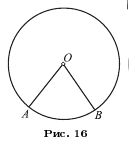
\includegraphics{mppics/ris-16}
\caption{}\label{1938/ris-16}
\bigskip
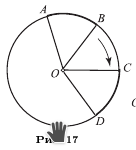
\includegraphics{mppics/ris-17}
\caption{}\label{1938/ris-17}
\end{wrapfigure}


\paragraph{Центральный угол.}\label{1938/17}
Угол ($AOB$, рис.~\ref{1938/ris-16}), образованный двумя радиусами окружности, называется \rindex{центральный угол}центральным углом;
о таком угле и дуге, заключённой между его сторонами, говорят, что они \textbf{соответствуют} друг другу.

Центральные углы по отношению к соответствующим им дугам обладают следующими двумя свойствами.

\textbf{\emph{В одном круге или в равных кругах.}}

1) \textbf{\emph{Если центральные углы равны, то и соответствующие им дуги равны.}}

2) Обратно.
\textbf{\emph{Если дуги равны, то и соответствующие им центральные углы равны.}}


Пусть $\angle AOB=\angle COD$ (рис.~\ref{1938/ris-17}), покажем, что дуги $AB$ и $CD$ также равны.
Вообразим, что сектор $AOB$ мы повернули вокруг центра $O$ в направлении, указанном стрелкой, настолько, чтобы радиус $OA$ совпал с $OC$.
Тогда, вследствие равенства углов, радиус $OB$ совместится с $OD$;
значит, совместятся и дуги $AB$ и $CD$, то есть
они будут равны.

Второе свойство также легко обнаружить наложением.

}

\paragraph{Градусы дуговой и угловой.}\label{1938/18}
Вообразим, что какая-нибудь окружность разделена на 360 равных частей и ко всем точкам деления проведены радиусы.
Тогда вокруг центра образуются 360 центральных углов, которые, как соответствующие равным дугам, должны быть равны между собой.
Каждая из полученных таким образом на окружности дуг называется \rindex{градус}\textbf{дуговым градусом}, а каждый из образовавшихся при центре углов называется \textbf{угловым градусом}.
Значит, можно сказать, что дуговой градус есть $\tfrac1{360}$ часть окружности,
а угловой градус есть центральный угол, соответствующий дуговому градусу.

Градусы (дуговые и угловые) подразделяются ещё на 60 равных частей, называемых \rindex{минута}\textbf{минутами}, а минуты подразделяются ещё на 60 равных частей, называемых \rindex{секунда}\textbf{секундами}.

\begin{figure}[!ht]
\centering
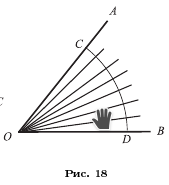
\includegraphics{mppics/ris-18}
\caption{}\label{1938/ris-18}
\end{figure}

Пусть $AOB$ есть какой-нибудь угол (рис.~\ref{1938/ris-18}).
Опишем между его сторонами с центром в вершине $O$ дугу $CD$ произвольного радиуса;
тогда угол $AOB$ будет центральным углом, соответствующим дуге $CD$.
При этом угол измеряется соответствующей ему дугой; то есть в угле содержится столько угловых градусов, минут и секунд, сколько в соответствующей ему дуге содержится дуговых градусов, минут и секунд.
Если, например, в дуге $CD$ содержится $20{,}57$ градусов или, что то же самое, 20 градусов 34 минуты 12 секунд,%
\footnote{Поскольку \[20{,}57=20\tfrac{57}{100}=20+\tfrac{34}{60}+\tfrac{12}{60\cdot 60}.\]}
 то и в угле $AOB$ заключается 20 градусов 34 минуты 12 секунд угловых, что принято выражать так:
$\angle AOB = 20{,}57\degree = 20\degree 34'12''$ обозначая знаками $\degree$, $'$ и $''$ соответственно градусы, минуты и секунды.

Величина углового градуса не зависит от радиуса окружности.
Действительно, если сложить 360 угловых градусов по правилу, указанному в §~\ref{1938/15}, то получим полный угол при центре окружности.
Каков бы ни был радиус окружности, этот полный угол будет один и тот же.
Значит, можно сказать, что угловой градус составляет $\tfrac1{360}$ часть полного угла;
это мера угла, определяющая его величину независимо от радиуса окружности.
Число угловых градусов в данном угле принимают за меру наклона одной стороны угла к другой.

Поскольку число 360 имеет много делителей,
градусы удобны для работы с дробными долями полного угла.
Тем не менее основной единицей измерения углов считается \textbf{радиан};
он будет определён в §~\ref{extra/radians}. 
Кроме градусов и радиан употребляются и другие единицы для измерения углов, например \textbf{прямой угол}, \textbf{оборот} равный полному углу и
\textbf{град} равный сотой доле прямого угла.
%существенное изменение

\begin{figure}[!ht]
\centering
\ \ \ \ \includegraphics{mppics/transportir-19}
\caption{}\label{1938/ris-19}
\end{figure}

%%%%overfull
\paragraph{Транспортир.}\label{1938/20}
Для измерения углов употребляется особый прибор — \rindex{транспортир}\textbf{транспортир}.
Этот прибор (рис.~\ref{1938/ris-19}) представляет собой полукруг, дуга которого разделена на $180\degree $.
Чтобы измерить угол $DCE$, накладывают на него прибор так, чтобы центр полукруга совпадал с вершиной угла, а радиус $CB$ был расположен по стороне $CE$.
Тогда число градусов, содержащееся в дуге, заключённой между сторонами угла $DCE$, покажет его величину.
При помощи транспортира можно также начертить угол, содержащий данное число градусов.

\paragraph{Прямой, острый и тупой углы.}\label{1938/21}
Угол в $90\degree$ (составляющий, следовательно, половину развёрнутого угла или четверть полного угла) называют \rindex{прямой угол}\textbf{прямым углом};
угол, меньший прямого, называют \rindex{острый угол}\textbf{острым}, а угол, больший прямого, но меньший развёрнутого, называют \rindex{тупой угол}\textbf{тупым} (рис.~\ref{1938/ris-20})

\begin{figure}[!ht]
\centering
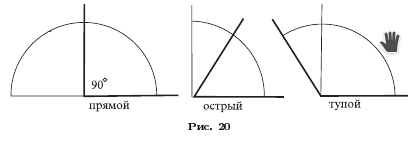
\includegraphics{mppics/ris-20}
\caption{}\label{1938/ris-20}
\end{figure}

Конечно, \textbf{\emph{все прямые углы}}, как содержащие одинаковое число градусов, \textbf{\emph{равны между собой}}.
На чертежах прямой угол принято обозначать квадратиком, как показано на рис.~\ref{1938/ris-20}.

\subsection*{Смежные и вертикальные углы}



\paragraph{Смежные углы и их свойства.}\label{1938/22}
Два угла ($AOB$ и $BOC$, рис.~\ref{1938/ris-21}) называются \rindex{смежные углы}\textbf{смежными}, если одна сторона у них общая, а две другие стороны составляют продолжение одна другой.

Так как такие углы в сумме составляют развёрнутый угол, то \textbf{\emph{сумма двух смежных углов равна $\bm{180\degree}$}}.

\begin{figure}[!ht]
\begin{minipage}{.48\textwidth}
\centering
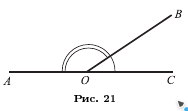
\includegraphics{mppics/ris-21}
\end{minipage}\hfill
\begin{minipage}{.48\textwidth}
\centering
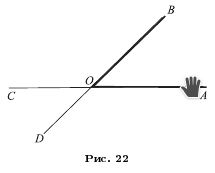
\includegraphics{mppics/ris-22}
\end{minipage}

\medskip

\begin{minipage}{.48\textwidth}
\centering
\caption{}\label{1938/ris-21}
\end{minipage}\hfill
\begin{minipage}{.48\textwidth}
\centering
\caption{}\label{1938/ris-22}
\end{minipage}
\vskip-4mm
\end{figure}

Для каждого данного угла можно построить два смежных с ним угла.
Например, для угла $AOB$ (рис.~\ref{1938/ris-22}), продолжив сторону $AO$, мы получим один смежный угол $BOC$.
\emph{Два угла, $BOC$ и $AOD$, смежные с одним и тем же углом $AOB$, равны между собой,} так как каждый из них дополняет угол $AOB$ до $180\degree$.

\begin{wrapfigure}{r}{35 mm}
\vskip-0mm
\centering
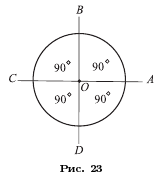
\includegraphics{mppics/ris-23}
\caption{}\label{1938/ris-23}
\end{wrapfigure}

Если угол $AOB$ прямой (рис.~\ref{1938/ris-23}), то есть если он содержит $90\degree$, то и каждый из смежных с ним углов $COB$ и $AOB$ должен быть также прямой, так как он содержит в себе $180\degree-90\degree$, то есть $90\degree$;
четвёртый угол $COB$ тоже должен быть прямым, так как три угла $AOB$, $BOC$ и $AOB$ составляют в сумме $270\degree$ и, следовательно, от $360\degree$ на долю четвёртого угла $COB$ остаётся тоже $90\degree$.
Таким образом:
\emph{если при пересечении двух прямых \emph{($AC$ и $BD$, рис.~\ref{1938/ris-23})} один из четырёх углов окажется прямой, то и остальные три угла должны быть прямые.}

\paragraph{Перпендикуляр и наклонная.}\label{1938/23}
Общая сторона ($OB$) двух смежных углов называется \rindex{наклонная}\textbf{наклонной} к прямой ($AC$), на которой лежат две другие стороны, в том случае, когда смежные углы не равны между собой (рис.~\ref{1938/ris-24});
в том же случае, когда смежные углы равны (рис.~\ref{1938/ris-25}) и когда, следовательно, каждый из углов есть прямой, общая сторона называется \rindex{перпендикуляр}\textbf{перпендикуляром} к прямой, на которой лежат две другие стороны.
Общая вершина ($O$) в первом случае называется \rindex{основание! наклонной}\textbf{основанием наклонной}, во втором случае — \textbf{основанием перпендикуляра}.

\begin{figure}[!ht]
\begin{minipage}{.48\textwidth}
\centering
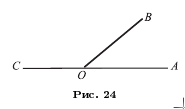
\includegraphics{mppics/ris-24}
\end{minipage}\hfill
\begin{minipage}{.48\textwidth}
\centering
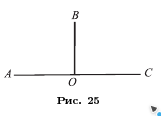
\includegraphics{mppics/ris-25}
\end{minipage}

\medskip

\begin{minipage}{.48\textwidth}
\centering
\caption{}\label{1938/ris-24}
\end{minipage}\hfill
\begin{minipage}{.48\textwidth}
\centering
\caption{}\label{1938/ris-25}
\end{minipage}
\vskip-4mm
\end{figure}

Две прямые ($AC$ и $BD$, рис.~\ref{1938/ris-23}), пересекающиеся между собой под прямым углом, называются взаимно \rindex{перпендикулярные прямые}\textbf{перпендикулярными}.
Что прямая $AC$ перпендикулярна к прямой $BD$, записывают так: $AC\perp BD$.

{\small

\smallskip

\mbox{\so{Замечания}.}
1) Если перпендикуляр к прямой $AC$ (рис.~\ref{1938/ris-25}) приходится проводить из точки $O$, лежащей на этой прямой, то говорят, что этот перпендикуляр надо «восстановить» к прямой $AC$, а если требуется перпендикуляр провести из точки $B$, лежащей вне прямой, то говорят, что его надо \so{опустить} на прямую (всё равно:
вниз или вверх, или вбок).
%1) Если перпендикуляр к прямой $AC$ (рис.~\ref{1938/ris-25}) приходится проводить из точки $O$, лежащей на этой прямой, то говорят, что этот перпендикуляр надо «восстановить» к прямой $AC$, а если требуется перпендикуляр провести из точки $B$, лежащей вне прямой, то говорят, что его надо "опустить" на прямую (всё равно:
%вниз или вверх, или вбок).
% либо 
%1) Если перпендикуляр к прямой $AC$ (рис.~\ref{1938/ris-25}) приходится проводить из точки $O$, лежащей на этой прямой, то говорят, что этот перпендикуляр надо  \so{восстановить} к прямой $AC$, а если требуется перпендикуляр провести из точки $B$, лежащей вне прямой, то говорят, что его надо \so{опустить} на прямую (всё равно:
%вниз или вверх, или вбок).
%для единообразия оформления?

2) Очевидно, что из всякой точки данной прямой можно к этой прямой восстановить перпендикуляр и притом только один.

}

\begin{wrapfigure}{r}{38 mm}
\centering
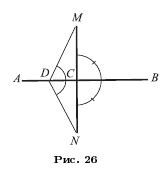
\includegraphics{mppics/ris-26}
\caption{}\label{1938/ris-26}
\end{wrapfigure}

\paragraph{}\label{1938/24}
Докажем, что \textbf{\emph{из всякой точки, лежащей вне прямой, можно опустить на эту прямую перпендикуляр и только один}}.

Пусть дана какая-нибудь прямая $AB$ (рис.~\ref{1938/ris-26}) и вне её произвольная точка $M$;
требуется показать, что, во-первых, из этой точки можно опустить на прямую $AB$ перпендикуляр и, во-вторых, что этот перпендикуляр может быть только один.

Вообразим, что мы перегнули чертёж;
по прямой $AB$ так, чтобы верхняя его часть упала на нижнюю.
Тогда точка $M$ займёт некоторое положение $N$.
Отметив это положение, приведём чертёж;
в прежний вид и затем соединим точки $M$ и $N$ прямой.
Убедимся, что полученная прямая $MN$ перпендикулярна к $AB$, а всякая иная прямая, исходящая из $M$, например $MD$, не перпендикулярна к $AB$.
Для этого перегнём чертёж вторично.
Тогда точка $M$ снова совместится с $N$, а точки $C$ и $D$ останутся на своих местах;
следовательно, прямая $MC$ совпадёт с $NC$, а $MD$ с $ND$.
Из этого следует, что $\angle MCB = \angle BCN$ и $\angle MDC = \angle CDN$.

Но углы $MCB$ и $BCN$ смежные и, как теперь видим, равные;
следовательно, каждый из них есть \so{прямой}, а потому $MN\z\perp AB$.
Так как линия $MDN$ не прямая (потому что не может быть двух различных прямых, соединяющих точки $M$ и $N$), то сумма двух равных углов $MDC$ и $CDN$ \so{не равна} $180\degree$;
поэтому угол $MDC$ не есть прямой, и, значит, $MD$ не перпендикулярна к $AB$.
Таким образом, другого перпендикуляра из точки $M$ на прямую $AB$ опустить нельзя.


\paragraph{Чертёжный угольник.}\label{1938/25} 
Для построения перпендикуляра к данной прямой очень удобен угольник — чертёжный инструмент в виде треугольника у которого один из углов делается прямым.
Чтобы провести перпендикуляр к прямой $AB$ (рис.~\ref{1938/ris-27}) через точку $D$, взятую вне прямой, приставляют линейку к прямой $AB$, к линейке угольник, а затем, придерживая линейку рукой, двигают угольник вдоль линейки до тех пор, пока другая сторона прямого угла не пройдёт через точку $D$, затем проводят прямую $CE$.
Точно также поступают если точка $D$ лежит на прямой $AB$.


\begin{figure}[h]
\begin{minipage}{.48\textwidth}
\centering
\includegraphics{mppics/ris-wood-27}
\end{minipage}\hfill
\begin{minipage}{.48\textwidth}
\centering
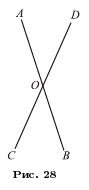
\includegraphics{mppics/ris-28}
\end{minipage}

\medskip

\begin{minipage}{.48\textwidth}
\centering
\caption{}\label{1938/ris-27}
\end{minipage}\hfill
\begin{minipage}{.48\textwidth}
\centering
\caption{}\label{1938/ris-28}
\end{minipage}
\vskip-4mm
\end{figure}


\paragraph{Вертикальные углы и их свойство.}\label{1938/26}
Два угла называются \rindex{вертикальные углы}\textbf{вертикальными}, если стороны одного составляют продолжение сторон другого.
Так, при пересечении двух прямых $AB$ и $CD$ (рис.~\ref{1938/ris-28}) образуются две пары вертикальных углов:
$AOD$ и $COB$, $AOC$ и $DOB$ (и четыре пары смежных углов).

{
\sloppy

\textbf{\emph{Два вертикальных угла равны между собой}} (например, $\angle AOD \z= \angle BOC$), так как каждый из них есть смежный с одним и тем же углом (с~$\angle DOB$ или с~$\angle AOC$), а такие углы, как мы видели (§~\ref{1938/22}), равны друг другу.

}

\paragraph{Замечания об углах, имеющих общую вершину.}\label{1938/27}
Об углах, имеющих общую вершину, полезно помнить следующие простые истины.

\begin{figure}[h]
\begin{minipage}{.48\textwidth}
\centering
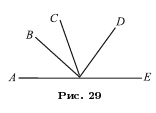
\includegraphics{mppics/ris-29}
\end{minipage}\hfill
\begin{minipage}{.48\textwidth}
\centering
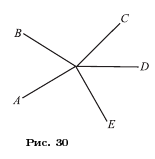
\includegraphics{mppics/ris-30}
\end{minipage}

\medskip

\begin{minipage}{.48\textwidth}
\centering
\caption{}\label{1938/ris-29}
\end{minipage}\hfill
\begin{minipage}{.48\textwidth}
\centering
\caption{}\label{1938/ris-30}
\end{minipage}
\vskip-4mm
\end{figure}

1) \emph{Если сумма нескольких углов ($AOB$, $BOC$, $COD$, $DOE$, рис.~\ref{1938/ris-29}), имеющих общую вершину, составляет развёрнутый угол, то она равна $180\degree$.}

2) \emph{Если сумма нескольких углов ($AOB$, $BOC$, $COD$, $DOE$, $EOA$ рис.~\ref{1938/ris-30}), имеющих общую вершину, составляет полный угол, то она равна  $360\degree$.}

3) \emph{Если два угла ($AOB$ и $BOC$, рис.~\ref{1938/ris-24}) имеют общую вершину ($O$) и общую сторону ($OB$) и в сумме составляют $180\degree$, то их две другие стороны ($AO$ и $OC$) составляют продолжение одна другой} (то есть такие углы будут смежными).


{\small

\subsection*{Упражнения}


\begin{enumerate}[noitemsep]
\item
Некоторый угол равен $38\degree 20'$;
найти величину смежного с ним угла.

\item
Два угла $ABC$ и $CBD$, имея общую вершину $B$ и общую сторону $BC$, расположены так, что они не покрывают друг друга;
угол $ABC \z= 100\degree20'$ , а угол $CBD = 79\degree 40'$.
Составляют ли стороны $AB$ и $BD$ прямую или ломаную.

\item
Построить какой-нибудь угол и при помощи транспортира и линейки провести его биссектрису.

\end{enumerate}

\smallskip
\so{Доказать}, что:

\begin{enumerate}[resume,noitemsep]
\item
Биссектрисы двух смежных углов взаимно перпендикулярны.

\item
Биссектрисы двух вертикальных углов составляют продолжение одна другой.

\item
Если при точке $O$ прямой $AB$ (рис.~\ref{1938/ris-28}) построим по разные стороны от $AB$ равные углы $AOB$ и $BOC$, то стороны их $OD$ и $OC$ составляют одну прямую.

\item
Если из точки $O$ (рис.~\ref{1938/ris-28}) проведём полупрямые $OA$, $OB$, $OB$, $OC$ так, что $\angle AOC = \angle DOB$ и $\angle AOD=\angle COD$, то $OD$ есть продолжение $OA$ и $OB$ есть продолжение $OC$.

\smallskip
\so{Указание}.
Надо применить §~\ref{1938/27}, 2 и 3.

\end{enumerate}

}
